\documentclass{article}
\usepackage{times}
\usepackage{graphicx}
\usepackage{subfigure}
\usepackage{natbib}
\usepackage{algorithm}
\usepackage{algorithmic}
\usepackage{hyperref}
\newcommand{\theHalgorithm}{\arabic{alorithm}}
\usepackage{icml2015}
\usepackage{multicol}
\usepackage{bbm}
\usepackage{amsmath}
\usepackage{hanging}
\usepackage{setspace}
\usepackage{etoolbox}
\usepackage{graphicx}
\AtBeginEnvironment{hangparas}{\singlespacing}
\AfterEndEnvironment{hangparas}{\addvspace{0.67\baselineskip}}
\icmltitlerunning{Final Project}
\begin{document}

\twocolumn[
\icmltitle{Final Project}
\icmlauthor{Joshua Rinaldi, Carlos Lawrence}{joshua.rinaldi@colorado.edu, carlos.lawrence@colorado.edu}
\vskip 0.3in
]

\begin{center}
Joshua Rinaldi, joshua.rinaldi@colorado.edu\\
Carlos Lawrence, carlos.lawrence@colorado.edu\\
Project GitHub Repository: https://github.com/Wopke123/tictactoe
\end{center} 
\vskip 0.3in

\begin{abstract}
One popular area of research in Machine Learning is teaching a computer how best to play a game. People have done this on games such as Super Mario World, Battleship and Brick Breaker. We set out to create a program that would play tic-tac-toe game that would learn as it played the game more on and be able to eventually beat a human player.
\end{abstract}

\section{Introduction}
When on Google, if one were to search for "Machine Learning Tic Tac Toe" a multitude of results would come up. There are numerous results that can be found which give tutorials on how to train a model to play tic tac toe. There are also some links that will take you to a tic tac toe game where you play against a machine. We wanted to do the same on our own, and then eventually train the model against itself, interested to see if both "players" would become equally proficient at the game, or if one player would become drastically better than the other. We started out by making our own implementation of tic tac toe and then later on added in a computer player using Reinforcement Learning to learn how to play the game and compete with both human and computer players.

\section{Related Works}
One person, Christopher J. MacLellan made a project that was almost exactly the same as what we set out to do, his process was different, but the end result was the same. There are also plenty of other examples readily available after an internet search where people have programmed a computer to play and learn how to play tic tac toe. In addition to this, there are multitudes of tic tac toe games where there is an option to play against a computer, and while we cannot say for sure if these games use Machine Learning, it can be a safe guess that there are some that do. \\
Machine Learning is not new to the video game world. As mentioned before, it is a very popular practice for a person to write a program to play a game as a project, there are also many video games in existence where the computer will learn how you play and how to counter your actions in the game. Implementation of Machine Learning into video games is something that can be fun for the developer, and make the game more challenging for the player.

\section{Playing Tic Tac Toe}
Our model uses the full game board state to determine the best next move. The state of the board is recorded as an array with a 0 for an unclaimed space, a -1 for a space claimed by the other player, and a 1 for a space claimed by the current player. Each player has a vector that represents the board in this manner, so Player 1's vector would be the inverse of player 2's, and it is this vector that is altered after each move. \\
As the game moves on, each player's history is also stored in a vector. The history is essentially a snapshot of the game board at the start of a player's turn, and the move that the player made at that turn. It is this vector of histories which is used by the computer to learn how to play the game. When the game has concluded, the history vector is used to update the bias vector for the given game state. \\
This knowledge base exists in a file and consists of every state the computer has seen to date, as well as a vector containing a weight for each square on the board, given the current state of the board. Before being trained, the file is empty. After each game that is run, this file is updated. Any previously unseen states are added to the file, and those states that are already in the have their weight vectors updated. Whenever the machine wins, the weights for the moves made at those states are rewarded. They are punished whenever the machine loses and a tie will reward both. Ties are rewarded to encourage the models to learn how to take the game to a tie. Statistically speaking, two expert players should be able to draw any game to a tie, so we wanted to encourage the model's ability to tie games as much as winning. In an attempt to improve our model, we focused on changing the update function for the bias vector, which would be used to actually allow assign new weights to different moves.  

\subsection{Linear Function}
This was the simplest of the functions that we tried. In the event of a win, we would add one point, in the event of a loss we would subtract one point. If there was a draw we would add one for both players. The issue with this function is that it allows for an unlimited upper and lower bound on the expected reward. The issue with this is that much larger numbers need to be stored, and this has the potential to get messy when the computer performs hundreds of thousands of training runs.

\subsection{First Sigmoid Function}
Following the linear function, we then normalized all of our results to fit within a range of (0, 1). This yielded numbers that were much easier to handle than our linear function. Another advantage of using this function is that it prevented over confidence in certain moves, something which can happen very easily operating under a linear function. However, we were hoping to have a range of (-1, 1) rather than a range of (0,1).

\subsection{Hyperbolic Tangential Functional}
The third function that we tried was a hyperbolic tangential function. The advantage that we got out of this function was that it yielded the range of (-1, 1) that we were looking for. However, this function greatly increased the complexity of our code and slowed down the process by a factor of 6. Because of this decreased performance, we opted to go back to a sigmoid function.

\subsection{Second Sigmoid Function}
The new function that we used was a modified version of the sigmoid function. It is:
\[\frac{1}{1 + e^{(-(a-0.5) * 5)}}\]

The reason that we opted to use this function as opposed to a traditional sigmoid function is that a traditional sigmoid function would cluster the majority of our results between 0.5 and 0.7, and as the model ran longer and longer, the grouping of these results would begin to get tighter and tighter around 0.6. Instead, with the function that we use it keeps our results even distributed in the range of (-1, 1) and allows for much cleaner numbers to work with. The reason that this works better for our model is that in our model we can look at the highest value in our weight vector and take into consideration all values around it. This will allow for the model to choose options other than those with the absolute highest weight and therefore avoid getting stuck on certain moves, preventing overfitting. It is far easier to differentiate these values under the new sigmoid function, with a wider range of values, than to do so on the original sigmoid function which had a much tighter spread.

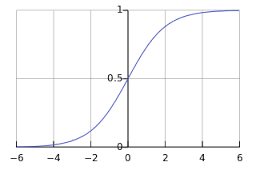
\includegraphics[scale=0.7]{sigmoid.png} \\
Graph of a regular Sigmoid Function. \\
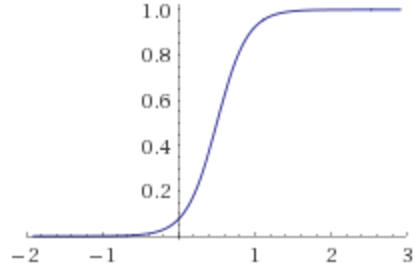
\includegraphics[scale=0.85]{newSigmoid.png} \\
Graph of our Sigmoid Function

\section{Analysis}
With no real bench mark against which to compare our program it is difficult to compare the end results of some of our tests. There are certainly inefficiencies in how we have written our model, which can be clearly seen in that after several hundred thousand runs it is still very easy to beat the computer, and the computer still tends to make moves that a human player would never make, for example, not blocking an obvious win for an opponent, or not taking a game winning move when available. However, there is a marked difference when playing against the model before and after training, and the model is capable of beating a human somewhat regularly.

\section{Future Work}
Moving forward there are a few things that would be interesting to look at. The first is that abilities of different algorithms, such as \textit{KNN}, where we could map out the board onto a nine dimensional space with each point being the move ending in the result of a win or tie and classifying the next move to take based on that. This could also be done as neural network, something which we avoided doing now for the sake of maintaining a grasp of what was going on in our model. This model also has the potential to be extended to other games such as Connect 4.

\section{Conclusion}
Using Reinforcement Learning we were able to make a model that could effectively learn how to play Tic Tac Toe by being trained against itself. We tried a few different methods of finding the weight for each move and in the end settled on using a modified Sigmoid Function. 

\section*{References}

\begin{hangparas}{0.3cm}{1}
MacLellan, C. (2016, March 27). Teaching a Computer to Play TicTacToe [Web blog post]. Retrieved December 8, 2016, from http://www.christopia.net/blog/teaching-a-computer-to-play-tictactoe.
\end{hangparas}
\begin{hangparas}{0.3cm}{1}
Ostermiller, S. (Unknown). Tic-Tac-Toe Strategy. [Web blog post]. Retrieved December 8, 2016, from http://blog.ostermiller.org/tic-tac-toe-strategy.
\end{hangparas}
 
\end{document}